% Тип документа
\documentclass[a4paper,12pt]{extarticle}

% Шрифты, кодировки, символьные таблицы, переносы
\usepackage{cmap}
\usepackage[T2A]{fontenc}
\usepackage[utf8x]{inputenc}
\usepackage[russian]{babel}

% Это пакет -- хитрый пакет, он нужен но не нужен
\usepackage[mode=buildnew]{standalone}

\usepackage
	{
		% Дополнения Американского математического общества (AMS)
		amssymb,
		amsfonts,
		amsmath,
		amsthm,
		% misccorr,
		% 
		% Графики и рисунки
		wrapfig,
		graphicx,
		subcaption,
		float,
		tikz,
		tikz-3dplot,
		caption,
		csvsimple,
		color,
		booktabs,
		pgfplots,
		pgfplotstable,
		geometry,
		% 
		% Таблицы, списки
		makecell,
		multirow,
		indentfirst,
		%
		% Интегралы и прочие обозначения
		ulem,
		esint,
		esdiff,
		% 
		% Колонтитулы
		fancyhdr,
	}  


% Обводка текста в TikZ
\usepackage[outline]{contour}

% Увеличенный межстрочный интервал, французские пробелы
\linespread{1.3} 
\frenchspacing 

 
\usetikzlibrary
	{
		decorations.pathreplacing,
		decorations.pathmorphing,
		patterns,
		calc,
		scopes,
		arrows,
		fadings,
		through,
		shapes.misc,
		arrows.meta,
		3d,
		quotes,
		angles,
		babel
	}


\tikzset{
	force/.style=	{
		>=latex,
		draw=blue,
		fill=blue,
				 	}, 
	%				 	
	axis/.style=	{
		densely dashed,
		blue,
		line width=1pt,
		font=\small,
					},
	%
	th/.style=	{
		line width=1pt},
	%
	acceleration/.style={
		>=open triangle 60,
		draw=magenta,
		fill=magenta,
					},
	%
	inforce/.style=	{
		force,
		double equal sign distance=2pt,
					},
	%
	interface/.style={
		pattern = north east lines, 
		draw    = none, 
		pattern color=gray!60,
					},
	cross/.style=	{
		cross out, 
		draw=black, 
		minimum size=2*(#1-\pgflinewidth), 
		inner sep=0pt, outer sep=0pt,
					},
	%
	cargo/.style=	{
		rectangle, 
		fill=black!70, 
		inner sep=2.5mm,
					},
	%
	caption/.style= {
		midway,
		fill=white!20, 
		opacity=0.9
					},
	%
	}

\newenvironment{tikzpict}
    {
	    \begin{figure}[htbp]
		\centering
		\begin{tikzpicture}
    }
    { 
		\end{tikzpicture}
		% \caption{caption}
		% \label{fig:label}
		\end{figure}
    }


\newcommand{\vbLabel}[3]{\draw ($(#1,#2)+(0,5pt)$) -- ($(#1,#2)-(0,5pt)$) node[below]{#3}}
\newcommand{\vaLabel}[3]{\draw ($(#1,#2)+(0,5pt)$) node[above]{#3} -- ($(#1,#2)-(0,5pt)$) }

\newcommand{\hrLabel}[3]{\draw ($(#1,#2)+(5pt,0)$) -- ($(#1,#2)-(5pt,0)$) node[right, xshift=1em]{#3}}
\newcommand{\hlLabel}[3]{\draw ($(#1,#2)+(5pt,0)$) node[left, xshift=-1em]{#3} -- ($(#1,#2)-(5pt,0)$) }



\newcommand\zi{^{\,*}_i}
\newcommand\sumn{\sum_{i=1}^{N}}

\tikzset{
	coordsys/.style={scale=1.8,x={(1.1cm,-0cm)},y={(0.5cm,1cm)}, z={(0cm,0.8cm)}},
	coordsys/.style={scale=1.5,x={(0cm,0cm)},y={(1cm,0cm)}, z={(0cm,1cm)}}, 
	coordsys/.style={scale=1.5,x={(1cm,0cm)},y={(0cm,1cm)}, z={(0cm,0cm)}}, 
}

\usepgfplotslibrary{units}


% Draw line annotation
% Input:
%   #1 Line offset (optional)
%   #2 Line angle
%   #3 Line length
%   #5 Line label
% Example:
%   \lineann[1]{30}{2}{$L_1$}

\newcommand{\lineann}[4][0.5]{%
    \begin{scope}[rotate=#2, blue,inner sep=2pt, ]
        \draw[dashed, blue!40] (0,0) -- +(0,#1)
            node [coordinate, near end] (a) {};
        \draw[dashed, blue!40] (#3,0) -- +(0,#1)
            node [coordinate, near end] (b) {};
        \draw[|<->|] (a) -- node[fill=white, scale=0.8] {#4} (b);
    \end{scope}
}

\newcommand{\lineannn}[4][0.5]{%
    \begin{scope}[rotate=#2, blue,inner sep=2pt, ]
        \draw[dashed, blue!40] (0,0) -- +(0,#1)
            node [coordinate, near end] (a) {};
        \draw[dashed, blue!40] (#3,0) -- +(0,#1)
            node [coordinate, near end] (b) {};
        % \draw[color=white, color=blue] (a) -- node[fill=white, scale=0.8] {#4} (b);
        \draw[->|] (a)++(-0.3,0) -- (a);
        \draw[->|] (b)++(0.3,0) coordinate (xx) -- (b);
        \draw (xx) node[fill=white, scale=0.8, right] {#4};
    \end{scope}
}

% Круговая стрелка относительно центра (дуга из центра)
\tikzset{
  pics/carc/.style args={#1:#2:#3}{
    code={
      \draw[pic actions] (#1:#3) arc(#1:#2:#3);
    }
  },
  dash/.style={
  	dash pattern=on 5mm off 5mm
  }
}

% Среднее <#1>
\newcommand{\mean}[1]{\langle#1\rangle}

\pgfplotsset{
    % most recent feature set of pgfplots
    compat=newest,
}

% const прямым шрифтом
\newcommand\ct[1]{\text{\rmfamily\upshape #1}}
\newcommand*{\const}{\ct{const}}


\usepackage[europeanresistors,americaninductors]{circuitikz}

% Style to select only points from #1 to #2 (inclusive)
\pgfplotsset{select/.style 2 args={
    x filter/.code={
        \ifnum\coordindex<#1\def\pgfmathresult{}\fi
        \ifnum\coordindex>#2\def\pgfmathresult{}\fi
    }
}}


\usepackage{array}



%%%%%%%%%%%%%%%%%%%%%%%%%%%%%%%%%%%%%%%%%%%%%%%%%
\makeatletter
\newif\if@gather@prefix 
\preto\place@tag@gather{% 
  \if@gather@prefix\iftagsleft@ 
    \kern-\gdisplaywidth@ 
    \rlap{\gather@prefix}% 
    \kern\gdisplaywidth@ 
  \fi\fi 
} 
\appto\place@tag@gather{% 
  \if@gather@prefix\iftagsleft@\else 
    \kern-\displaywidth 
    \rlap{\gather@prefix}% 
    \kern\displaywidth 
  \fi\fi 
  \global\@gather@prefixfalse 
} 
\preto\place@tag{% 
  \if@gather@prefix\iftagsleft@ 
    \kern-\gdisplaywidth@ 
    \rlap{\gather@prefix}% 
    \kern\displaywidth@ 
  \fi\fi 
} 
\appto\place@tag{% 
  \if@gather@prefix\iftagsleft@\else 
    \kern-\displaywidth 
    \rlap{\gather@prefix}% 
    \kern\displaywidth 
  \fi\fi 
  \global\@gather@prefixfalse 
} 
\newcommand*{\beforetext}[1]{% 
  \ifmeasuring@\else
  \gdef\gather@prefix{#1}% 
  \global\@gather@prefixtrue 
  \fi
} 
\makeatother
%%%%%%%%%%%%%%%%%%%%%%%%%%%%%%%%%%%%%%%%%%%%%%%%%

\geometry		
	{
		left			=	2cm,
		right 			=	2cm,
		top 			=	3cm,
		bottom 			=	3cm,
		bindingoffset	=	0cm
	}

%%%%%%%%%%%%%%%%%%%%%%%%%%%%%%%%%%%%%%%%%%%%%%%%%%%%%%%%%%%%%%%%%%%%%%%%%%%%%%%

\def\labauthors{Понур К.А., Сарафанов Ф.Г., Сидоров Д.А.}
\def\labgroup{420}
\def\labnumber{222}
\def\labtheme{Изучение разряда неоновой лампы}

	%применим колонтитул к стилю страницы
\pagestyle{fancy} 
	%очистим "шапку" страницы
\fancyhead{} 
	%слева сверху на четных и справа на нечетных
\fancyhead[R]{\labauthors} 
	%справа сверху на четных и слева на нечетных
\fancyhead[L]{Отчёт по лабораторной работе №\labnumber} 
	%очистим "подвал" страницы
\fancyfoot{} 
	% номер страницы в нижнем колинтуле в центре
\fancyfoot[C]{\thepage} 

%%%%%%%%%%%%%%%%%%%%%%%%%%%%%%%%%%%%%%%%%%%%%%%%%%%%%%%%%%%%%%%%%%%%%%%%%%%%%%%

\renewcommand{\contentsname}{Оглавление}

\usepackage{tocloft}
% \renewcommand{\cftpartleader}{\cftdotfill{\cftdotsep}} % for parts
% \renewcommand{\cftsectiondotsep}{\cftdotsep}% Chapters should use dots in ToC
\renewcommand{\cftsecleader}{\cftdotfill{\cftdotsep}}
%\renewcommand{\cftsecleader}{\cftdotfill{\cftdotsep}} % for sections, if you really want! (It is default in report and book class (So you may not need it).
% ---------
% \newcommand{\cftchapaftersnum}{.}%
% \usepackage{titlesec}
% \titlelabel{\thetitle.\quad}
\usepackage{secdot}
\sectiondot{subsection}

\begin{document}

\def\labauthors{Понур К.А., Сарафанов Ф.Г., Сидоров Д.А.}
\def\labgroup{420}
\def\labnumber{210}
\def\labtheme{Исследование линейных двухполюсников и четырёхполюсников}
\renewcommand{\vec}{\mathbf}
\renewcommand{\Re}{\operatorname{Re}}
\renewcommand{\Im}{\operatorname{Im}}

\begin{titlepage}

\begin{center}

{\small\textsc{Нижегородский государственный университет имени Н.\,И. Лобачевского}}
\vskip 1pt \hrule \vskip 3pt
{\small\textsc{Радиофизический факультет}}

\vfill

{\Large Отчет по лабораторной работе №\labnumber\vskip 12pt\bfseries \labtheme}
	
\end{center}

\vfill
	
\begin{flushright}
	{Выполнили студенты \labgroup\ группы\\ \labauthors}%\vskip 12pt Принял:\\ Менсов С.\,Н.}
\end{flushright}
	
\vfill
	
\begin{center}
	Нижний Новгород, \the\year
\end{center}

\end{titlepage}



\tableofcontents
\newpage
\section{Схема №1. Последовательная $RC$ -- цепочка}
\begin{center}
	\documentclass[border=1pt]{standalone}
\usepackage[europeanresistors,americaninductors]{circuitikz}

\begin{document}
	
      \begin{circuitikz}[]

            \draw (0,0) to [short,o-] (0,2)
            to [R] (-2,2)
            to [capacitor] (-4,2)
            to [short,-o] (-4,0)
            ; 
	\end{circuitikz}
\end{document}
\end{center}

Рассчитаем импеданс конденсатора методом комплексных амплитуд.
\begin{equation}
	\hat{U}=U_0 e^{i(\omega t+\phi_U)}
\end{equation}
Величину $\hat{U_0}=U_0e^{i\phi_U}$ будем называть комплексной амплитудой напряжения
\begin{equation}
	I=C\diff{U}{t}
\end{equation}
Отсюда получаем:
\begin{equation}
	\hat{I}=U_0\,\omega i C\exp(i\omega t+\phi_U)
\end{equation}
И комплексная амплитуда тока:
\begin{equation}
	\hat{I_0}=U_0i\omega C e^{i\phi_U}
\end{equation}
Получаем комплексный импеданс конденсатора
\begin{equation}
	\hat{z}_C=\frac{\hat{U_0}}{\hat{I_0}}=\frac{U_0e^{i\phi_U}}{U_0i\omega C e^{i\phi_U}}=\frac{1}{i\cdot\omega C}
\end{equation}
Нетрудно получить, что $\hat{z}_R=R$. Тогда импеданс $RC$ --цепочки
\begin{equation}
	\hat{z}=\frac{1}{i\cdot\omega C}+R
\end{equation}
\begin{equation}
	z=\sqrt{
		\frac{1}{\omega^2 C^2}	
		+R^2
	}=
	\sqrt{
		\frac{1}{\omega^2 C^2}	
		+\frac{R^2\omega^2 C^2}{\omega^2 C^2}
	}=\frac{\sqrt{1+(\omega RC)^2}}{\omega C}
\end{equation}
Экспериментально можно снимать зависомость $U_{13}\equiv U_\text{вх}$ и $U_{23}\equiv U_\text{вых}$ от частоты. Из закона Ома найдем тогда импеданс цепочки.
\begin{gather}
	\hat{J}_{13}=\hat{J}_{23} \quad\Rightarrow\quad
	\frac{\hat{U}_{13}}{\hat{z}}=\frac{\hat{U}_{23}}{R}
\end{gather}
Взяв по модулю получим нужное соотношение
\begin{equation}
	z=\frac{U_\text{вх}}{U_\text{вых}}R
\end{equation}
Также найдем зависимость разности фаз от частоты:
\begin{equation}
	|\tan\phi| = |\frac{\Im\hat{z}}{\Re\hat{z}}|=
	|\frac{
		-(\omega C)^{-1}
	}{
		R
	}|=
	\frac{
		1
	}{
		\omega RC
	}	
\end{equation}
%!TEX root=../polypole.tex
\begin{table}[H]
	    \caption{Результаты эксперимента для первой схемы}
	    \label{tab:chem1}
	    \pgfkeys{/pgf/number format/.cd,
		fixed,  1000 sep={\,}}
\newlength\Colsep
\setlength\Colsep{10pt}
% \xdef\Table{data/i.tsv}
	     \xdef\C{5e-8}
\xdef\R{13000}  
\pgfplotstableset{
	% multicolumn names, % allows to have multicolumn names
	% header=has colnames,
	dec sep align,
	col sep=tab, % the seperator in our .csv file
	fixed zerofill, 
	precision=4,
    create on use/omega/.style={
        create col/expr={
        \thisrow{Fr}*2*3.14
        }
    },	 
    create on use/z/.style={
        create col/expr={
        13000*\thisrow{Uin}/\thisrow{Uout}
        }
    },				
	columns/z/.style={
		column name={$z$, Ом},
		precision=0		
	},	
	columns/Fr/.style={
		column name={$\nu$, Гц},
		precision=0,		
	},		
	columns/omega/.style={
		column name={$\omega$, Гц},
		precision=0,		
	},	
	columns/a/.style={
		column name={$a$},
		precision=1,		
	},		
	columns/b/.style={
		column name={$b$},
		precision=1,		
	},					
	columns/Uin/.style={
		column name={$U_{in}$, В},
		precision=3,		
		% column type/.add={|}{},
	},
	columns/Uout/.style={
		column name={$U_{in}$, В},
		precision=3,				
		% column type/.add={|}{},
	},
	columns/phi/.style={
		column name={$\phi$, рад},
		precision=2,				
		% column type/.add={|}{},
	},
	columns/dphi/.style={
		column name={$\Delta\phi$, рад},
		precision=2,				
		% column type/.add={|}{},
	},	
	columns/tanphi/.style={
		column name={$\tan\phi$},
		precision=3,				
		% column type/.add={|}{},
	},		
	empty cells with={\textbf{--}},
	every head row/.style={
	before row={\toprule},
	after row={
		\midrule}
		},
	every last row/.style={after row=\bottomrule},
	every row/.style={after row=\midrule}, 
	columns={Fr,omega,a,b,phi,tanphi,Uin,Uout,z},		
	% dec zerofill
	% fixed,fixed zerofill,
	% precision=3
	% every even column/.style={
	% 	% column type/.add={>{\columncolor[gray]{.8}}}{}
	% },
	% every even row/.style={
	% 	before row={\rowcolor[gray]{0.95}}
	% },	
	}
	\centering
	\pgfplotstabletypeset[]{data/chem1.tsv}

\end{table}
\begin{figure}[H]
	\centering
	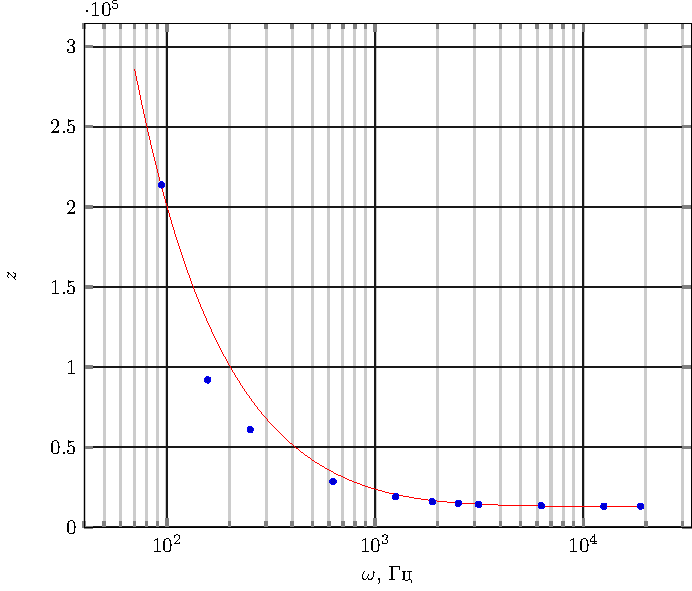
\includegraphics[width=0.85\textwidth]{img/chem1_z}
	\caption{Зависимость $z(\omega)$ для последовательной $RC$--цепочки}
	\label{fig:figure1}
\end{figure}
\begin{figure}[H]
	\centering
	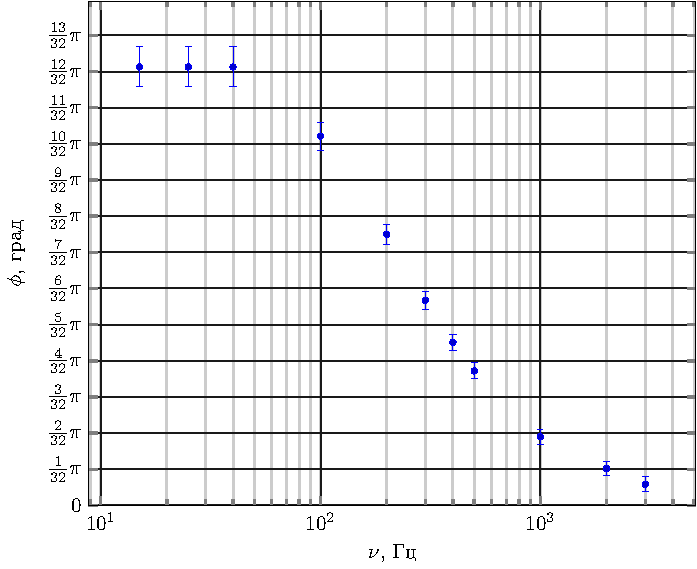
\includegraphics[width=0.85\textwidth]{img/chem1_phi} 
	\caption{Зависимость $\tan\phi(\omega)$ для последовательной $RC$--цепочки}
	\label{fig:figure1}
\end{figure}
\section{Вторая схема}
\begin{center}
\documentclass[border=1pt]{standalone}
\usepackage[europeanresistors,americaninductors]{circuitikz}

\begin{document}
	
      \begin{circuitikz}[]

            \draw (0,0) to [short,o-] (0,2)
            to [R] (-2,2)
            to [inductor] (-4,2)
            to [short,-o] (-4,0)
            ; 
	\end{circuitikz}
\end{document}
\end{center}

\begin{equation}
	\hat{I}=I_0e^{i(\omega t+\phi_I)}
\end{equation}
\begin{equation}
	U=L\diff{I}{t}
\end{equation}
\begin{equation}
	\hat{U}=I_0i\omega L e^{i(\omega t +\phi_I)}
\end{equation}
Отсюда
\begin{equation}
	\hat{z}=i\omega L
	\end{equation}

\begin{figure}[H]
	\centering
	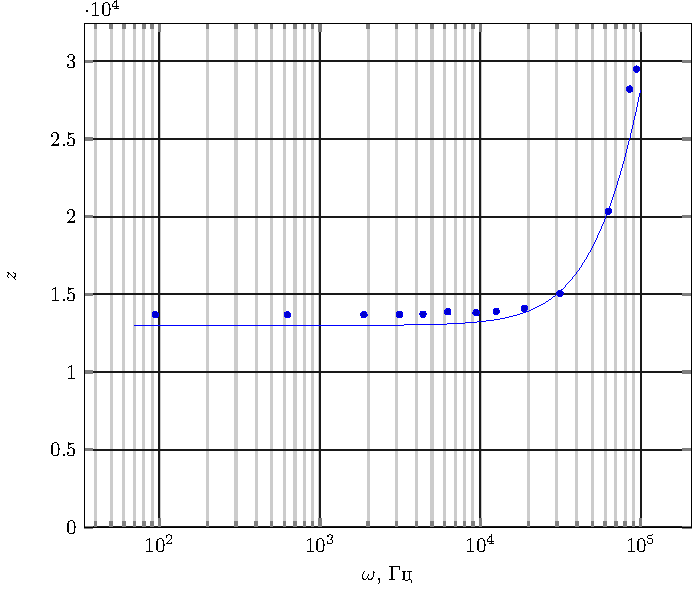
\includegraphics[width=0.85\textwidth]{img/chem2_z}
	\caption{Зависимость $z(\omega)$ для последовательной $LC$--цепочки}
	\label{fig:figure1}
\end{figure}
\begin{figure}[H]
	\centering
	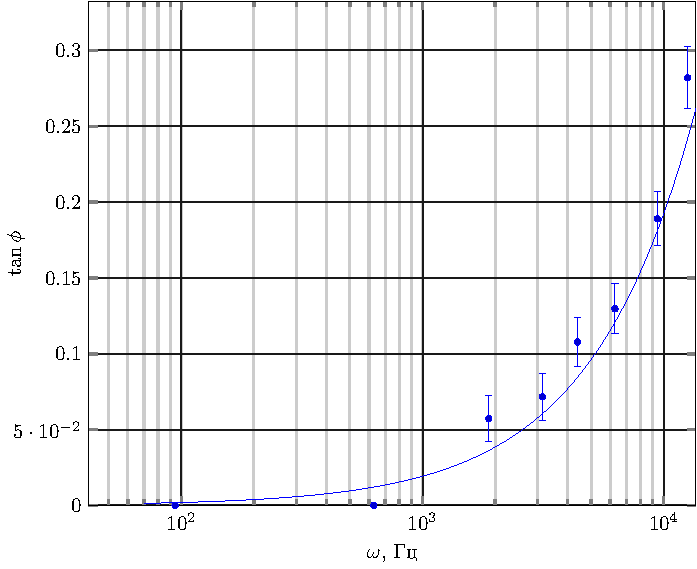
\includegraphics[width=0.85\textwidth]{img/chem2_phi} 
	\caption{Зависимость $\tan\phi(\omega)$ для последовательной $LC$--цепочки}
	\label{fig:figure1}
\end{figure}

\section{Третья схема}
\begin{center}
\documentclass[border=1pt]{standalone}
\usepackage[europeanresistors,americaninductors]{circuitikz}

\begin{document}
	
      \begin{circuitikz}[]

            \draw (0,0) to [short,o-](2,0)
            to [R=$R_1$] (2,-2) 
            to (1.5,-2)
            to [capacitor,C,  l_=$C$] (1.5,-4)
            to (2,-4)
            to (2,-5)
            to [short,-o] (0,-5);       
            \draw (2,-2) 
            to (2.5,-2) 
            to [R=$R_2$] (2.5,-4)
            to (2,-4);
	\end{circuitikz}
\end{document}
\end{center}
Сначала расчитаем импеданс параллельно соединенных конденсатора и резистора $R_2$
\begin{equation}
	\frac{1}{\hat{z_0}}=\frac{1}{R_2}+i\omega C
\end{equation}
\begin{equation}
	\hat{z_0}=\frac{R_2}{1+i \omega CR_2}
\end{equation}
Комплексный импеданс всей схемы будет равен:
\begin{equation}
	\hat{z}=\hat{z_0}+R_1=\frac{R_2}{1+i \omega R_2C}+R_1=
	\frac{R_2(1-i \omega R_2C)}{1+(\omega R_2C)^2}+R_1
\end{equation}
Отсюда
\begin{equation}
	\tan\phi = \frac{\Im\hat{z}}{\Re\hat{z}}=
	\frac{
		-\frac{\omega R_2^2C}{1+(\omega R_2C)^2}
	}{
		\frac{R_2+R_1+R_1(\omega R_2C)^2}{1+(\omega R_2C)^2}
	}=
	\frac{
		-\omega R_2^2C
	}{
		R_2+R_1+R_1(\omega R_2C)^2
	}	
\end{equation}


\section{Четвертая схема}
\begin{center}
\documentclass[border=1pt]{standalone}
\usepackage[europeanresistors,americaninductors]{circuitikz}

\begin{document}
	
      \begin{circuitikz}[]

            \draw  (0,0) to [short,o-] (2,0)
            to [R=$R_1$] (2,-2) 
            to (1.5,-2)
            to [L] (1.5,-4)
            to (2,-4)
            to (2,-5)
            to [short,-o] (0,-5);       
            \draw (2,-2) 
            to (2.5,-2) 
            to [R=$R_2$] (2.5,-4)
            to (2,-4);
	\end{circuitikz}
\end{document}
\end{center}
Рассчитаем импеданс параллельно соединенных катушки и резистора $R_2$
\begin{equation}
	\frac{1}{\hat{z_1}}=\frac{1}{R_2}+\frac{1}{i\omega L}
\end{equation}
\begin{equation}
	\hat{z_1}=\frac{R_2\omega^2L^2+iR_2^2\omega L}{R_2+\omega L}
\end{equation}
А импеданс всей схемы:
\begin{equation}
	\hat{z_0}=\frac{R_2\omega^2L^2}{R_2+\omega L} + R_1+i\frac{iR_2^2\omega L}{R_2+\omega L}
\end{equation}


\section{Пятая схема}
\begin{center}
\documentclass[border=1pt]{standalone}
\usepackage[europeanresistors,americaninductors]{circuitikz}

\begin{document}
	
      \begin{circuitikz}[]
      \ctikzset {label/align = straight }
            \draw (0,0) to [short,o-](0,3)
            to (3,3)
            to (3,2);
            \draw (0,-1) to [short,o-](0,-4) 
            to (3,-4) 
            to (3,-3);


            \draw (3,2) to [capacitor,l_=$C_1$](0.5,-0.5) %левая ветка
            to [R,l_=$R_1$](3,-3);
            \draw (3,2) to [R, l^=$R_2$] (5.5,-0.5) %правая ветка
            to [capacitor,l^=$C_2$](3,-3);
            \draw (0.5,-0.5) to [short,-o] (2,-0.5);
            \draw   (5.5,-0.5) to [short,-o](4,-0.5);
            	\end{circuitikz}
\end{document}
\end{center}



\section{Шестая схема}
\begin{center}
\documentclass[border=1pt]{standalone}
\usepackage[europeanresistors,americaninductors]{circuitikz}
\tikzset{
  pics/carc/.style args={#1:#2:#3}{
    code={
      \draw[pic actions] (#1:#3) arc(#1:#2:#3);
    }
  }
}

\begin{document}
	
      \begin{circuitikz}[]
      \draw (0,0) to [short,o-*,C=$C$](4,0)
      to [short,*-,C=$C$] ++(4,0)
      to [short,*-,C=$C$] ++(4,0)
      to  [short,-o] ++(2,0);

      \draw (0,-2) node  {$U_{in}$};
      \draw (14,-2) node  {$U_{out}$};

      \draw[thick] (2,-2) pic[red, -latex]{carc=-150:150:1.3cm} node {$J_1$};
      \draw[thick] (6,-2) pic[red, -latex]{carc=-150:150:1.3cm} node {$J_2$};
      \draw[thick] (10,-2) pic[red, -latex]{carc=-150:150:1.3cm} node {$J_3$};

      \draw (0,-4) to [short,o-](4,-4)
      to  [short,*-](8,-4)
      to  [short,*-](12,-4)
      to  [short,-o] (14,-4);

      \draw (4,0) to [R=$R$](4,-4);
      \draw (8,0) to [R=$R$](8,-4);
      \draw (12,0) to [short,*-*,R=$R$](12,-4);

      \end{circuitikz}
\end{document}
\end{center}


	\end{document}


